\section{Numerical Experiments}\label{sec:exp} 
We  now show via experiments that gates indeed play a central role in deep learning. For this we use the DGN setup (\Cref{fig:ablation}) to create models in the $4$ regimes namely DL, FL, FR-II and FR-DI. In each of the $4$ regimes, we create  combinatorially many models via a) permutation of the layers when the copied from the feature to the value network, and b) setting the input to the value network to $\mathbf{1}$ (in training and testing), i.e., a tensor with all its entries to be $1$. We observe that in all the $4$ regimes, the models are robust to the combinatorial variations.

\textbf{Setup:} Datasets are MNIST and CIFAR-10. For CIFAR-10, we use \Cref{fig:ablation} with $3\times 3$  windows and $128$ filters in each layer. For MNIST, we use FC instead of the convolutional layers.  All the FC-DNNs and CNNs are trained with `\emph{Adam}'  [\citenum{adam}] (step-size $=3\cdot 10^{-4}$ , batch size $=32$). We use $\beta=10$ in the DL regime.

\textbf{Reporting of Statistics:} The results are summarised in \Cref{fig:ablation}. For FC-DNN and CNN, in each of the $4$ regimes, we train $48= 2 (\xv=x / \xv=\mathbf{1}) \times 24(\text{layer permutations})$ models. Each of these models are trained to almost $100\%$ accuracy and the test performance is taken to be the best obtained in a given run. Each of the $48$ models is run only once. In all the cases the mean and deviation are reported.
\begin{figure}[b]
\begin{minipage}{0.64\textwidth}
\resizebox{\textwidth}{!}{
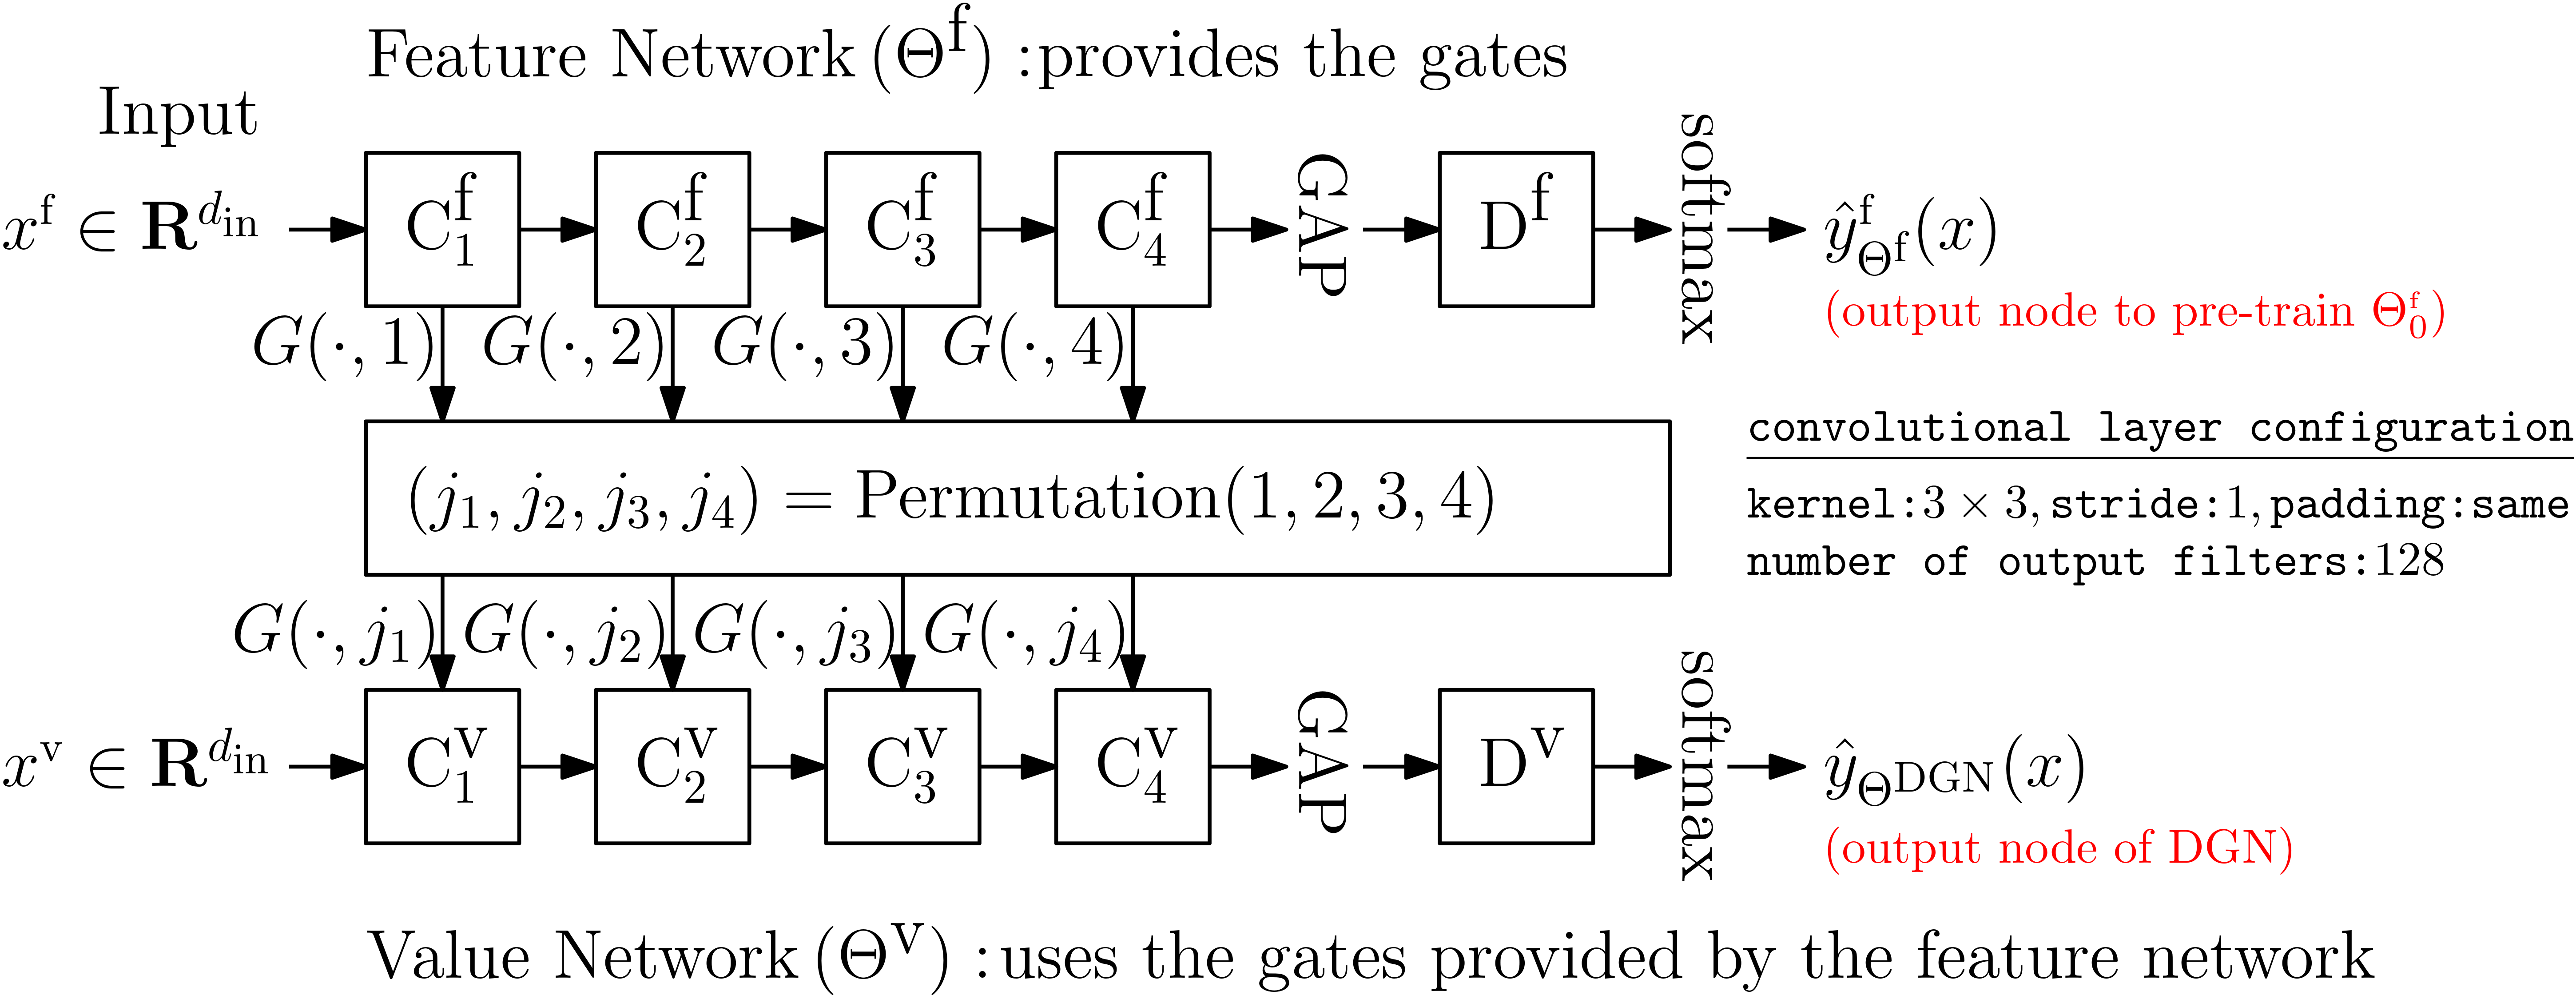
\includegraphics[scale=0.5]{figs/ablation.png}
}
\end{minipage}
\begin{minipage}{0.35\columnwidth}
\small
\resizebox{\columnwidth}{!}{
\begin{tabular}{|c|c|c|c|}\hline
&FC& CNN & ResNet\\\hline
%FR-II& $94.10\pm0.27\%$ & $67.53\pm0.73\%$\\\hline
%FR-DI& $94.06\pm0.25\%$ & $67.6\pm0.74\%$\\\hline
%DL& $98.14\pm0.07\%$ & $77.59\pm0.59\%$\\\hline
%FL& $98.62\pm0.05\%$ & $79.37\pm0.29\%$\\\hline
%ReLU& $\%$ & $\%$\\\hline
FR-II& $94.1\%$ & $67.5\%$ &$89.8\%$\\\hline
FR-DI& $94.1\%$ & $67.6\%$& $89.8\%$ \\\hline
DL& $98.1\%$ & $77.6\%$& $92.4\%$ \\\hline
FL& $98.6\%$ & $79.4\%$& $92.5\%$\\\hline
ReLU& $98.5\%$ & $80.4\%$& $93.1\%$\\\hline
\end{tabular}
}
\,In all cases, standard deviation was less than $0.5\%$. MNIST for FC, CIFAR-10 for CNN and ResNet.
\end{minipage}
\begin{comment}
\begin{minipage}{0.45\columnwidth}
\small
\resizebox{\columnwidth}{!}{
\begin{tabular}{|c|c|c|c|}\hline
& MNIST (FC)& CIFAR-10 (CNN) & CIFAR-10 (ResNet)\\\hline
%FR-II& $94.10\pm0.27\%$ & $67.53\pm0.73\%$\\\hline
%FR-DI& $94.06\pm0.25\%$ & $67.6\pm0.74\%$\\\hline
%DL& $98.14\pm0.07\%$ & $77.59\pm0.59\%$\\\hline
%FL& $98.62\pm0.05\%$ & $79.37\pm0.29\%$\\\hline
%ReLU& $\%$ & $\%$\\\hline
FR-II& $94.1\pm0.3\%$ & $67.5\pm0.7\%$ &$89.8\pm0.1\%$\\\hline
FR-DI& $94.1\pm0.3\%$ & $67.6\pm0.7\%$& $89.8\pm0.2\%$ \\\hline
DL& $98.1\pm0.1\%$ & $77.6\pm0.6\%$& $92.4\pm0.1\%$ \\\hline
FL& $98.6\pm0.1\%$ & $79.4\pm0.3\%$& $92.5\pm0.5\%$\\\hline
ReLU& $98.5\pm0.1\%$ & $80.4\pm0.3\%$& $93.1\pm0.1\%$\\\hline
\end{tabular}
}
\end{minipage}

\begin{minipage}{0.28\textwidth}
\resizebox{\columnwidth}{!}{
\begin{tabular}{|l|l|}\hline
Regimes & $\Tf$\\\hline
FR-II & R, NT\\\hline
FR-DI & R, NT, $\Tf_0=\Tv_0$\\\hline
FL & PT, NT\\\hline
DL & R, T\\\hline
\end{tabular}
}
\resizebox{\columnwidth}{!}{
\begin{tabular}{|l|l|}\hline
Mode	& Input\\\hline
Image	& $\xv=\xf=x$\\\hline
`All-Ones' & $\xf=x,\xv=\mathbf{1}$\\\hline
\end{tabular}
}
\end{minipage}
\end{comment}
\caption{\small{$\textrm{C}_i^{\text{f}},\textrm{C}_i^{\text{v}},i\in[4]$ are the convolutional layers, which are followed by \emph{global-average-pooling} (GAP) layer then by a dense layer ($\textrm{D}^{\text{f}}$/$\textrm{D}^{\text{v}}$), and a softmax layer to produce the final logits.}} %`R',  `L', `T' and `NT' stand for random, learnt, trainable and non-trainable respectively.}}
\label{fig:ablation}
\end{figure}


$\bullet$ \textbf{Result Discussion:}  Recall that in regimes FR-II and FR-DI the gates are fixed and random, and only $\Tv$ are trained. In DL regime, both $\Tf$ and $\Tv$ are trained, and FL regime $\Tf$ is pre-trained and fixed, and only $\Tv$ is trained. In the following discussion, we compare the performance of the models in various regimes, along with the performance of CNTK of \cite{arora2019exact} ($77.43\%$ in CIFAR-10) and the performance of standard DNN with ReLU.  The main observations are listed below (those by \cite{ch2020neural} are also revisited for the sake of completeness). 

\indent\quad $1.$ \emph{Decoupling:} There is no performance difference between FR-II and FR-DI.% i.e., the decoupling the gates from the weights did not affect the performance in practice. 
Further, decoupled learning of gates (DL) performs significantly better than fixed random gates (FR), and the gap between standard DNN with ReLU and DL is less than $3\%$. This marginal performance loss seems to be worthy trade off for fundamental insights of \Cref{th:main} under the decoupling assumption.


\indent\quad $2.$ \emph{Recovery:} The fixed learnt regime  (FL) shows that using the gates of a pre-trained ReLU network, performance can be recovered by training the NPV. Also, by interpreting the input dependent component of a model to be the features and the input independent component to be the weights, it makes sense to look at the gates/NPFs as the hidden features and NPV as the weights.% (which can be re-trained).

\indent\quad $3.$ \emph{Random Gates:} FR-II does perform well in all the experiments (note that for a $10$-class problem, a random classifier would achieve only $10\%$ test accuracy). Given the observation that the gates are the true features, and the fact that is no learning in the gates in the fixed regime, and the performance of fixed random gates can be purely attributed to the in-built structure.

\indent\quad $4.$ \emph{Gate Learning:} We group the models into three sets where $S_1=\{$ ReLU, FL , DL$\}$, $S_2=\{$ FR$\}$ and $S_3=\{$ CNTK $\}$, and explain the difference in performance due to gate learning.
 $S_2$ and $S_3$ have no gate learning. However,  $S_3$ due to its infinite width has better averaging resulting in a well formed kernel and hence performs better than $S_2$ which is a finite width. Thus, the difference between $S_2$ and $S_3$ can be attributed to finite versus infinite width. Both $S_1$ and $S_2$ are finite width, and hence, conventional feature learning happens in both $S_1$ and $S_2$, but, $S_1$ with gate learning is better ($77.5\%$ or above in CIFAR-10) than $S_2$ ($67\%$ in CIFAR-10) with no gate learning. Thus neither finite width, nor the conventional feature learning explain the difference between $S_1$ and $S_2$. Thus, `gate learning' discriminates the regimes $S_1, S_2$ and $S_3$ better than the conventional feature learning view.

\indent\quad $5.$ \emph{Permutation and Input Invariance:} The performance (in all the $4$ regimes) is  robust to `all-ones' inputs. Note that in the `all-ones' case, the input information affects the models only via the gates. Here, all the entries of the input Gram matrix are identical, and the NPK depends only on $\Lambda$, which is the measure of sub-network active simultaneously for the various input pairs. The performance (in all the $4$ regimes) is also robust to permutation of the layers. This can be attributed to the product $\Pi_{l=1}^{(d-1)} H^{\text{lyr}}_{l,\Theta}$ of the layer level base kernels being order invariant.

\indent\quad $6.$ \emph{Visualisation:} \Cref{fig:permute} compares the hidden layer outputs of a standard DNN with ReLU with $4$ layers, and that of a DGN which copies the gates from the standard DNN, but, reverses the gating masks when applying to the value network. Also, the value network of the DGN was provided with a fixed random input (as shown in \Cref{fig:permute}). Both the models achieved about $80\%$ test accuracy, an otherwise surprising outcome, yet, as per the theory developed in this paper, a random input to the value network should not have much effect on performance, and this experiment confirms the same.
\FloatBarrier
\begin{figure}[h]
\resizebox{\columnwidth}{!}{
\includegraphics{visual-iclr/images/horse.png}
\includegraphics{visual-iclr/images/original/layer_1_0.png}
\includegraphics{visual-iclr/images/original/layer_1_1.png}
\includegraphics{visual-iclr/images/original/layer_2_0.png}
\includegraphics{visual-iclr/images/original/layer_2_1.png}
\includegraphics{visual-iclr/images/original/layer_3_0.png}
\includegraphics{visual-iclr/images/original/layer_3_1.png}
\includegraphics{visual-iclr/images/original/layer_4_0.png}
\includegraphics{visual-iclr/images/original/layer_4_1.png}
}\\
%\tiny\text{For each model, input is shown first and then starting from the first layer, the first $2$ filters of each of the $4$ layers are shown.}
\end{figure}
\FloatBarrier
\begin{figure}[h]
\resizebox{\columnwidth}{!}{
\includegraphics{visual-iclr/images/randinput.png}
\includegraphics{visual-iclr/images/permuted/layer_1_0.png}
\includegraphics{visual-iclr/images/permuted/layer_1_1.png}
\includegraphics{visual-iclr/images/permuted/layer_2_0.png}
\includegraphics{visual-iclr/images/permuted/layer_2_1.png}
\includegraphics{visual-iclr/images/permuted/layer_3_0.png}
\includegraphics{visual-iclr/images/permuted/layer_3_1.png}
\includegraphics{visual-iclr/images/permuted/layer_4_0.png}
\includegraphics{visual-iclr/images/permuted/layer_4_1.png}
}
\end{figure}


\subsection{DGN as a Lookup Table: Applying \Cref{th:main} to a pure memorisation task}\label{sec:mem}

In this section, we modify the DGN in \Cref{fig:dgn} into a memorisation network to solve a pure memorisation task. The objective of constructing the memorisation network is to understand the roles of depth and width in \Cref{th:main} in a simplified setting. In this setting, we show increasing depth till a point helps in training and increasing depth beyond it hurts training. 

\begin{definition}[Memorisation Network/Task]
Given a set of values $(y_s)_{s=1}^n\in  \R$, a memorisation network (with weights $\Theta\in\R^{\dnet}$) accepts $s\in[n]$ as its input and produces $\hat{y}_{\Theta}(s)\approx y_s$ as its output. The loss of the memorisation network is defined as $L_{\Theta}=\frac{1}{2}\sum_{s=1}^n (\hat{y}_{\Theta}(s)-y_s)^2$.
\end{definition}
\FloatBarrier
\begin{table}[h]
\centering
\begin{tabular}{| l |  l  |}\hline
Layer&  Memorisation Network\\\hline
Input  &$z_{\Theta}(0)=1$ \\
Pre-Activation & $q_{s,\Theta}(l)=\sum_{j}\Theta(i,j,l)\cdot z_{s,\Theta}(j,l-1)$\\
Hidden & $z_{s,\Theta}(i,l)=q_{s,\Theta}(i,l)\cdot G_{s}(i,l)$ \\
Final  Output & $\hat{y}_{\Theta}(s)=\sum_{j} \Theta(1,j,d) \cdot z_{s,\Theta}(j,d-1)$\\\hline
\end{tabular}
\caption{ Memorisation Network. The input is fixed and is equal to $1$. All the internal variables depend on the index $s$ and the parameter $\Theta$. The gating values $G_s(i,l)$ are external and independent variables.}
\label{tb:dgnmemo}
\end{table}

\textbf{Fixed Random Gating:} The memorisation network is described in \Cref{tb:dgnmemo}. In a memorisation network, the gates are \emph{fixed and random}, i.e., for each index $s\in[n]$, the gating values $G_{s}(i,l),\forall l\in[d-1], i\in[w] $ are sampled from $Ber(\mu), \mu\in(0,1)$ taking values in $\{0,1\}$,  and kept fixed throughout training. The input to the memorisation network is fixed as $1$, and since the gating is fixed and random there is a separate random sub-network to memorise each target $y_s\in\R$. The memorisation network can be used to memorise the targets  $(y_s)_{s=1}^n$ by training it using gradient descent by minimising the squared loss $L_{\Theta}$. In what follows, we let $K_0$ and $H_0$ to be the NTK and NPK of the memorisation network at initialisation.


\textbf{Performance of Memorisation Network:} From \Cref{prop:basic} we know that as $w\ra\infty$, the training error dynamics of the memorisation network follows:
\begin{align}
\dot{e}_t=-K_{0} e_t,
\end{align}
i.e., the spectral properties of $K_0$ (or $H_0$) dictates the rate of convergence of the training error to $0$. In the case of the memorisation network with fixed and random gates, we can calculate $\E{K_0}$ explicitly. 

\textbf{Spectrum of $H_0$:} The input Gram matrix $\Sigma$ is a $n\times n$ matrix with all entries equal to $1$ and its rank is equal to 1, and hence $H_0=\Lambda_0$. We can now calculate the properties of $\Lambda_0$. It is easy to check that $\mathbb{E}_{\mu}\left[\Lambda_0(s,s)\right]=(\mu w)^{(d-1)},\forall s\in[n]$ and $\mathbb{E}_{\mu}\left[\Lambda_0(s,s')\right]=(\mu^2 w)^{(d-1)},\forall s,s'\in[n]$.  For $\sigma=\sqrt{\frac{1}{\mu w}}$, and $\mathbb{E}_{\mu}\left[K_0(s,s)/d\right]=1$, and $\mathbb{E}_{\mu}\left[K_0(s,s')/d\right]=\mu^{(d-1)}$. 
\begin{figure}
\centering
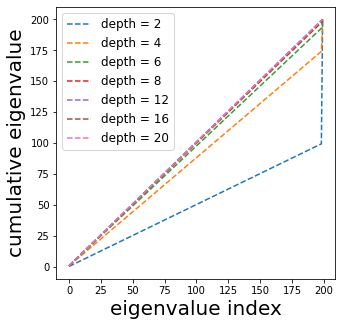
\includegraphics[scale=0.3]{figs/dgn-fra-ecdf-ideal-small.png}
\caption{Ideal spectrum of $\E{K_0}/d$ for a memorisation network for $n=200$.}
\label{fig:ideal-spectrum}
\end{figure}


\textbf{Why increasing depth till a point helps ?} 
We have:
%\comment{
\begin{align}\label{eq:mat}
\frac{\E{K_0}}{d}=\left[\begin{matrix}
1 &\mu^{d-1} &\ldots &\mu^{d-1} &\ldots\\ 
\ldots &1 &\ldots &\mu^{d-1} &\ldots\\ 
\ldots &\mu^{d-1} &\ldots &1 &\ldots \\
\ldots &\mu^{d-1} &\ldots &\mu^{d-1} &1\\ 
\end{matrix}\right]
\end{align}
%}
i.e., all the diagonal entries are $1$ and non-diagonal entries are $\mu^{d-1}$. Now, let $\rho_i\geq 0,i \in [n]$ be the eigenvalues of $\frac{\E{K_0}}{d}$, and let $\rho_{\max}$ and $\rho_{\min}$ be the largest and smallest eigenvalues.  One can easily show that $\rho_{\max}=1+(n-1)\mu^{d-1}$ and corresponds to the eigenvector with all entries as $1$, and $\rho_{\min}=(1-\mu^{d-1})$ repeats $(n-1)$ times,  which corresponds to eigenvectors given by $[0, 0, \ldots, \underbrace{1, -1}_{\text{$i$ and $i+1$}}, 0,0,\ldots, 0]^\top \in \R^n$ for $i=1,\ldots,n-1$. Note that as $d\ra\infty$, $\rho_{\max},\rho_{\min}\ra 1$.

\textbf{Why increasing depth beyond a point hurts?} 
As the depth increases the variance of the entries $K_0(s,s')$ deviates from its expected value $\E{K_0(s,s')}$. Thus the structure of the Gram matrix degrades from \eqref{eq:mat}, leading to smaller eigenvalues.
%\FloatBarrier
\begin{figure}
\resizebox{\textwidth}{!}{
\begin{tabular}{cccc}
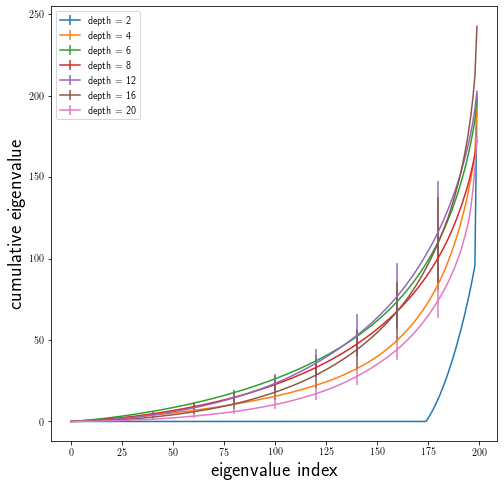
\includegraphics[scale=0.5]{figs/dgn-fra-ecdfbyd-w25.png}
&
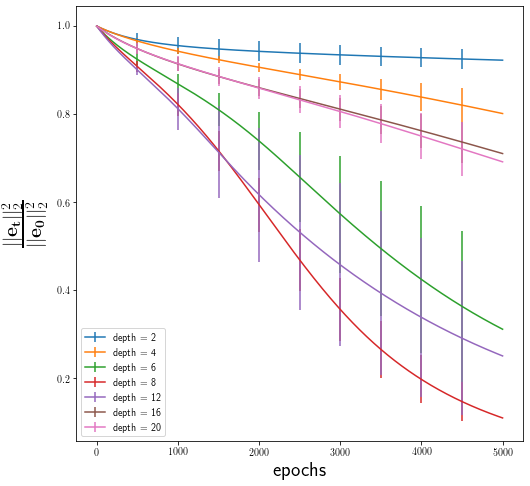
\includegraphics[scale=0.5]{figs/dgn-fra-conv-w25.png}
&
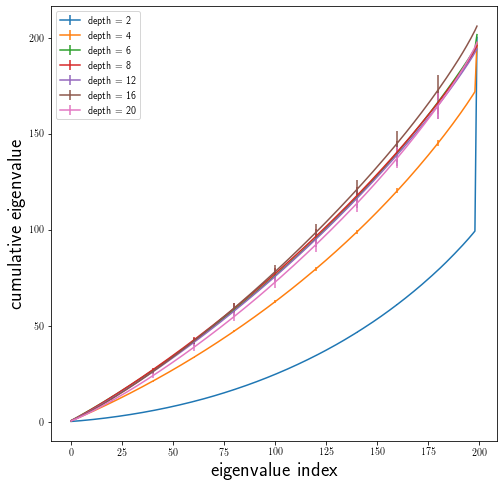
\includegraphics[scale=0.5]{figs/dgn-fra-ecdfbyd-w500.png}
&
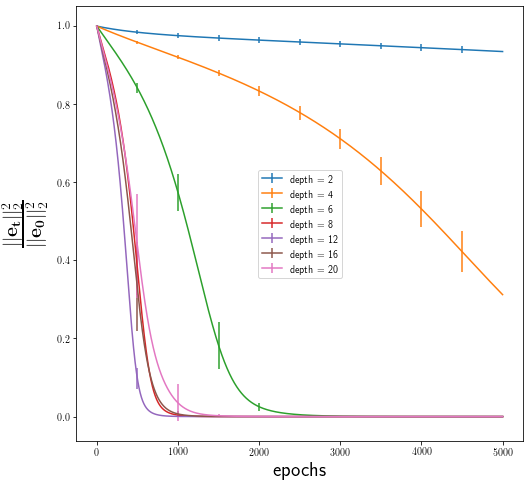
\includegraphics[scale=0.5]{figs/dgn-fra-conv-w500.png}
\end{tabular}
}
\caption{Shows the plots for the memorisation network with $\mu=\frac{1}{2}$ and $\sigma=\sqrt{\frac{2}{w}}$. The number of points to be memorised is $n=200$. The left most plot shows the e.c.d.f for $w=25$ and the second plot from the left shows the error dynamics during training for $w=25$. The second plot from the right shows the e.c.d.f for $w=500$ and the right most plot shows the error dynamics during training for $w=500$. All plots are averaged over $10$ runs.}
\label{fig:dgn-frg-gram-ecdf}
\end{figure}

\subsection{Experiment}
We set $n=200$, and $y_s\sim\text{Uniform}[-1,1]$. We look at the cumulative eigenvalue (e.c.d.f) obtained by first sorting the eigenvalues in ascending order then looking at their cumulative sum. The ideal behaviour (\Cref{fig:ideal-spectrum}) as predicted from theory is that for indices $k\in[n-1]$, the e.c.d.f should increase at a linear rate, i.e., the cumulative sum of the first $k$ indices is equal to $k(1-\mu^{d-1})$, and the difference between the last two indices is $1+(n-1)\mu^{d-1}$. In \Cref{fig:dgn-frg-gram-ecdf}, we plot the actual e.c.d.f for various depths $d=2,4,6,8,12,16,20$ and $w=25,500$ (first and third plots from the left in \Cref{fig:dgn-frg-gram-ecdf}). 

\textbf{Roles of depth and width:} In order to compare how the rate of convergence varies with the depth, we set the step-size $\alpha=\frac{0.1}{\rho_{\max}}$, $w=100$. We use the vanilla SGD-optimiser. Note the$ \frac{1}{\rho_{\max}}$ in the stepsize, ensures that the uniformity of maximum eigenvalue across all the instances, and the convergence should be limited by the smaller eigenvalues. We also look at the convergence rate of the ratio $\frac{\norm{e_t}^2_2}{\norm{e_0}^2_2}$. We notice that for $w=25$, increasing depth till $d=8$ improves the convergence, however increasing beyond $d=8$ worsens the convergence rate. For $w=500$, increasing the depth till $d=12$ improves convergence, and $d=16,20$ are worse than $d=12$.  %This matches with the depth phenomena observed in practical DNNs and also matches our theory.
